\documentclass[11pt]{scrartcl}
\usepackage{graphicx}
\graphicspath{{./}}
\usepackage[sexy]{evan}
\usepackage[normalem]{ulem}
\usepackage{hyperref}
\usepackage{mathtools}
\hypersetup{
    colorlinks=true,
    linkcolor=blue,
    filecolor=magenta,      
    urlcolor=cyan,
    pdfpagemode=FullScreen,
    }
\usepackage[most]{tcolorbox}
\renewcommand{\dangle}{\measuredangle}

\renewcommand{\baselinestretch}{1.5}

\addtolength{\oddsidemargin}{-0.4in}
\addtolength{\evensidemargin}{-0.4in}
\addtolength{\textwidth}{0.8in}
% \addtolength{\topmargin}{-0.2in}
% \addtolength{\textheight}{1in} 


\setlength{\parindent}{0pt}

\usepackage{pgfplots}
\pgfplotsset{compat=1.15}
\usepackage{mathrsfs}
\usetikzlibrary{arrows}

\title{Problem Set 2}
\author{Azzam Labib (IG: haxuv.world)}
\date{G5-6| Sunday, 23 June 2024}
\begin{document}
\maketitle

\section{Logical Reasoning (Paper A)}
\begin{enumerate}
\item $\frac{2}{3} \times 2.4 + 12.4 \times \frac{3}{4} = ?$
\begin{enumerate}[(A)]
    \item 9.9 \item 10.1 \item 10.9 \item 13.9
\end{enumerate}

\item Find the least common multiple of 15, 36, and 90.
\begin{enumerate}[(A)]
    \item 360 \item 270 \item 180 \item 120
\end{enumerate}

\item Determine the next figures of the following pattern.
\begin{figure}[h]
    \centering
    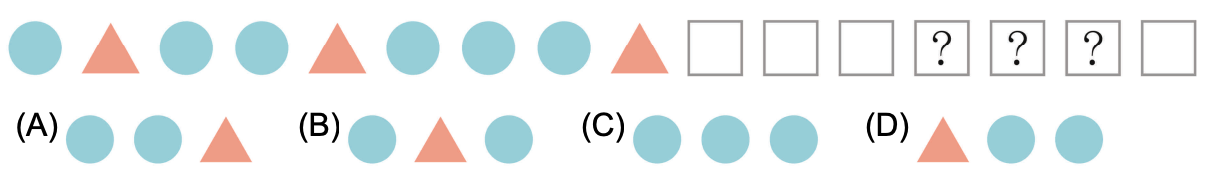
\includegraphics[scale=0.7]{StarGen/0Figure/wmi-2020-6a-num3.png}
\end{figure}

\newpage
\item If the two figures have the same areas, find the other side length of the figure on the right.
\begin{figure}[h]
    \centering
    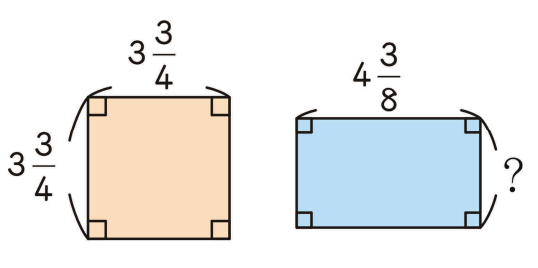
\includegraphics{StarGen/0Figure/wmi-2020-6a-two-rectangle.png}
\end{figure}
\begin{enumerate}[(A)]
    \item $\frac{9}{14}$ \item $3\frac{3}{4}$ \item $2\frac{7}{8}$ \item $3\frac{3}{14}$
\end{enumerate}

\item When Grandpa was 64 years old, Jenny was 4 years old. Now, Grandpa's age is 6 times the age of Jenny's. How old is Jenny now?
\begin{enumerate}[(A)]
    \item 8 \item 10 \item 12 \item 15
\end{enumerate}

\item The record shows the number and type of pitches $x$ that MLB pitcher Johnson threw in a game. What is $y$ approximately?
\begin{center}
    \begin{tabular}{|c|c|c|c|c|}
    \hline
    Fast ball & Slider & Curve & Change-up & Total\\
    \hline
    $48x$ & & $23x$ & & $126x$\\
    \hline
    38\% & 28\% & & $y$ & 100\%\\
    \hline
    \end{tabular}
\end{center}

\begin{enumerate}[(A)]
    \item 18\% \item 16\% \item 22\% \item 20\%
\end{enumerate}

\newpage
\item There are 27 students in class A. Tom was sick and missed the math test, so the average math score in class A was 69.5. The next day, Tom took the test, and the average math score in class A became 70. What was Tom's math test result?
\begin{enumerate}[(A)]
    \item 83 \item 82 \item 80 \item 78
\end{enumerate}

\item Given a large square on the right. Find $x$ in cm.
\begin{figure}[h]
    \centering
    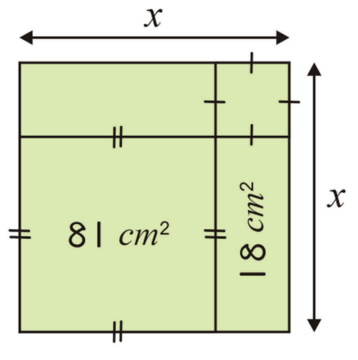
\includegraphics{StarGen/0Figure/wmi-2020-5a-square.png}
\end{figure}
\begin{enumerate}[(A)]
    \item 13 \item 12 \item 11 \item 10
\end{enumerate}

\item At 6:00 a.m., Ben drove from city A to city B at the speed of 90km/hr. After he arrived in city B, he rested for 4 hours, and then he drove back to city A on the same road at the speed of 120km/hr. Given that the distance between the two cities is 358km, when did Ben arrive in city A approximately?
\begin{enumerate}[(A)]
    \item 15:00 \item 16:00 \item 17:00 \item 18:00
\end{enumerate}

\newpage
\item Find the surface area of the figure on the right in cm$^2$.
\begin{figure}[h]
    \centering
    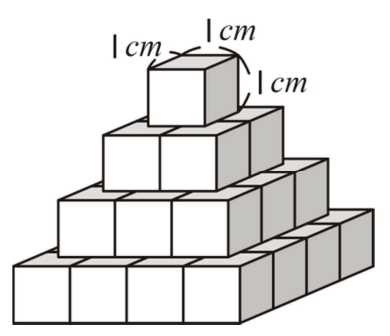
\includegraphics{StarGen/0Figure/wmi-2020-6a-pyramid-of-cubes.png}
\end{figure}
\begin{enumerate}[(A)]
    \item 56 \item 60 \item 72 \item 84
\end{enumerate}

\item $(1 - \frac{1}{3}) \div (1 - \frac{1}{4}) \div (1 - \frac{1}{5}) \div (1 - \frac{1}{6}) \div (1 - \frac{1}{7}) = ?$
\begin{enumerate}[(A)]
    \item $\frac{4}{7}$ \item $\frac{5}{8}$ \item $\frac{7}{9}$ \item $\frac{14}{9}$
\end{enumerate}

\item The speed of the small boat is 17km/hr, the speed of the large boat is 25km/hr, and the speed of the current is 3km/hr. The two boats start off at the same place, and the large boat starts off 1 hour later than the small boat. If both boats drive downstream, find the distance between the two boats 4 hours after the large boat start off in km.
\begin{enumerate}[(A)]
    \item 18 \item 15 \item 12 \item 9
\end{enumerate}

\newpage
\item Given that the length and the width of a rectangle are both integers which are larger than 1. Which cannot be the area of the rectangle?
\begin{enumerate}[(A)]
    \item 98 \item 111 \item 135 \item 101
\end{enumerate}

\item Find the volume of the solid. ($\pi = \frac{22}{7}$)
\begin{figure}[h]
    \centering
    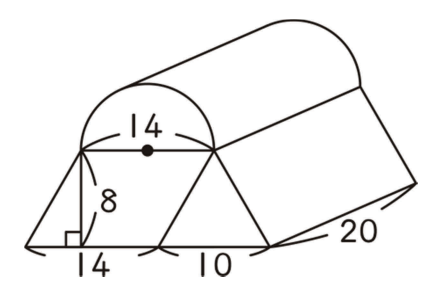
\includegraphics{StarGen/0Figure/wmi-2020-6a-volume-of-solid.png}
\end{figure}
\begin{enumerate}[(A)]
    \item 5000 \item 4840 \item 4580 \item 4060
\end{enumerate}

\newpage
\item Suppose $A$ and $B$ are numbers from $0--9$, and that follow the directions of the arrows will make $A$ become $B$, find $A + B$.
\begin{figure}[h]
    \centering
    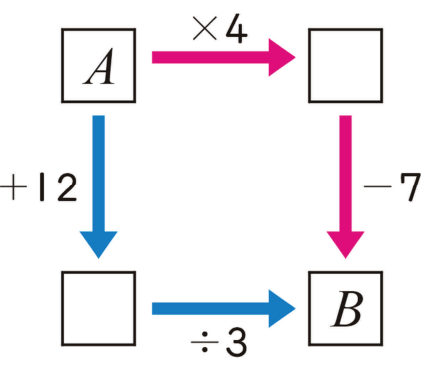
\includegraphics{StarGen/0Figure/wmi-2020-6a-diagram-operation.png}
\end{figure}
\begin{enumerate}[(A)]
    \item 6 \item 7 \item 8 \item 9
\end{enumerate}
\end{enumerate}

\section{Application (Paper B)}
\begin{enumerate}
    \item The weights of a bottle of juice, half a bottle of juice, and an empty bottle are shown below, respectively. Find the weight of an empty bottle in $g$.
    
    \begin{figure}[h]
        \centering
        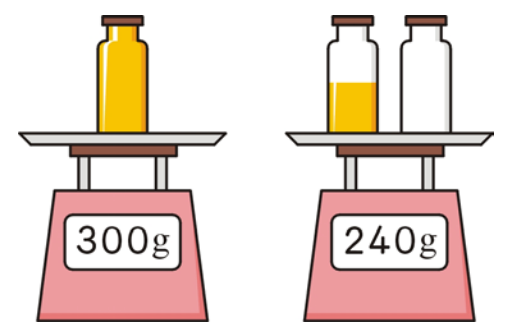
\includegraphics[scale=0.6]{StarGen/0Figure/wmi-2021-6b-bottle-juice.png}
    \end{figure}
    
    \item Find the smallest prime number $P$ to make $P + 2021$ a perfect square.
    
    \item What is the integer $n$ that makes the sum of $1 + 2 + 3 + \cdots + n$ a 3-digit number which is made up of the same digit?
    
    \item $\dfrac{\dfrac{1}{\frac{1}{10} - \frac{1}{12}}}{\dfrac{1}{\frac{1}{5} - \frac{1}{6}} + \dfrac{1}{\frac{1}{8} - \frac{1}{6}}} = ?$
    
    \item In the picture, the solid is formed by 2 cuboids. Find "?".
    
    \begin{figure}[h]
        \centering
        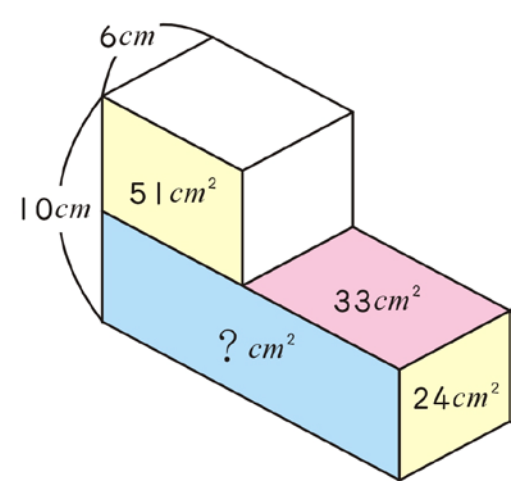
\includegraphics[scale=0.7]{StarGen/0Figure/wmi-2021-6b-cuboid.png}
    \end{figure}
    
    \item Arrange five positive integers in a row. Start from the second number, each number is not smaller than two times of its previous number. Given that the sum of the five numbers is 2021, find the smallest possible value of the last number in the row.
    
    \item When $1 + 11 + 11^2 + 11^3 + 11^4 + 11^5 + 11^6 + 11^7 + 11^8 + 11^9 + 11^{10}$ is divided by 100, what is the remainder?
    
    \item Below is a circular robot vacuum cleaner. Given that a circular side brush is installed on the edge of it, and the side brush cleans the floor by spinning clockwise around the robot vacuum cleaner. Find the maximum area that the side brush cleans when the robot vacuum cleaner pauses. ($\pi = 3.14$, round to the nearest integer)
    
    \begin{figure}[h]
        \centering
        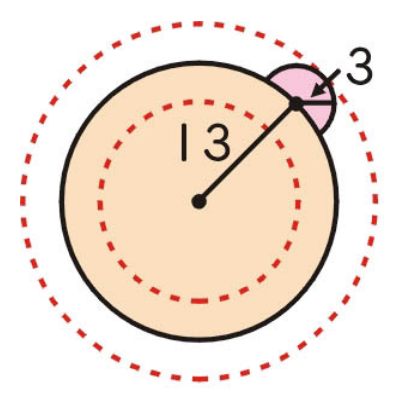
\includegraphics[scale=0.7]{StarGen/0Figure/wmi-2021-6b-robot-vacuum-cleaner.png}
    \end{figure}

    \newpage
    \item A rabbit wants to eat the carrot. If the rabbit has to pass all the squares once except the ones with stones, please write down numbers "1234" accordingly to help it get the carrot. Find the sum of the numbers on its way.
    
    \begin{figure}[h]
        \centering
        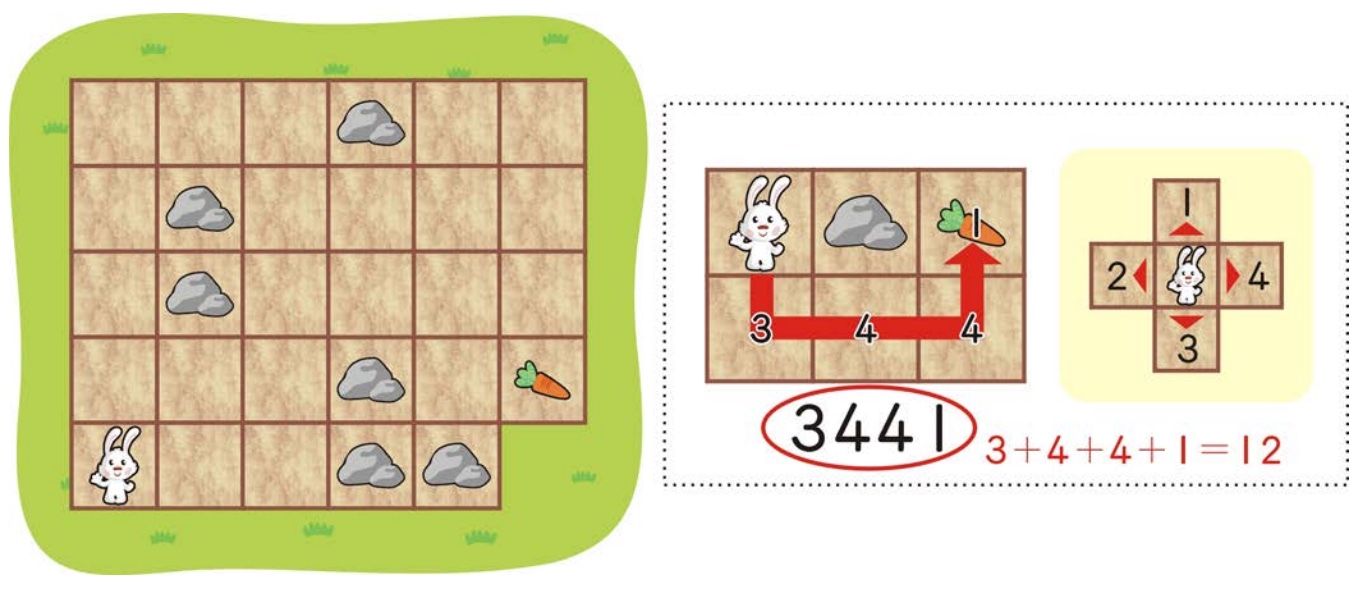
\includegraphics[scale=0.3]{StarGen/0Figure/wmi-2021-6b-rabbit-puzzle.jpeg}
    \end{figure}
    
    \item The picture shows a Sudoku game with numbers 1--5. If the small numbers in the center of the four squares must be the numbers which are written in these four squares, find the 5-digit number $ABCDE$.
    
    \begin{figure}[h]
        \centering
        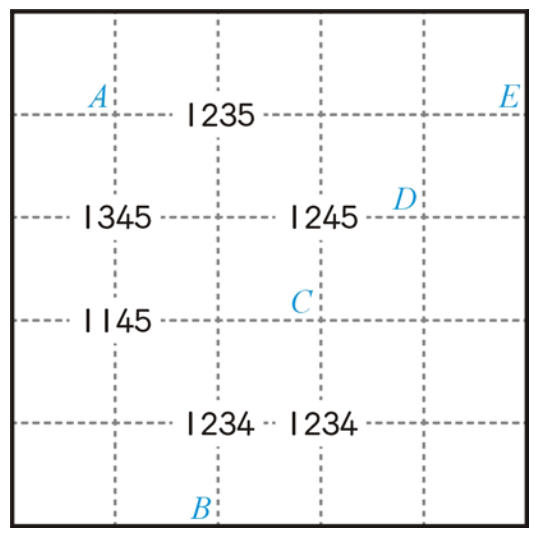
\includegraphics[scale=0.8]{StarGen/0Figure/wmi-2021-6b-sudoku-puzzle.png}
    \end{figure}
\end{enumerate}

\end{document}